\documentclass{article} % For LaTeX2e

\usepackage{amssymb}
\usepackage{bm}
\usepackage{clrscode3e}
\usepackage{float}
\usepackage{footmisc}
\usepackage{mathtools}

%icrl 2017
\usepackage{iclr2017_conference,times}
\usepackage{hyperref}
\usepackage{url}

\title{Efficient Calculation of Polynomial Features on Sparse Matrices}

%\author{Andrew Nystrom \\
%Savvysherpa Inc.\\
%6200 Shingle Creek Pkwy \\
%Suite 400 \\
%Minneapolis, MN 55430, USA \\
%\texttt{awnystrom@gmail.com} \\
%\And
%John F. Hughes \\
%Department of Computer Science \\
%Brown University \\
%Providence, RI \\
%\texttt{jfh@cs.brown.edu} \\
%}

\newcommand*\samethanks[1][\value{footnote}]{\footnotemark[#1]}
\renewcommand{\thefootnote}{\fnsymbol{thanks}}

\author{
  Nystrom, Andrew \\
  \texttt{awnystrom@gmail.com}
  \thanks{Now at Google}
  \ 
  \thanks{The authors contributed equally important and fundamental aspects of this work.}
  \and
  Hughes, John \\
  \texttt{jfh@cs.brown.edu}
  \footnotemark[2]
}

% The \author macro works with any number of authors. There are two commands
% used to separate the names and addresses of multiple authors: \And and \AND.
%
% Using \And between authors leaves it to \LaTeX{} to determine where to break
% the lines. Using \AND forces a linebreak at that point. So, if \LaTeX{}
% puts 3 of 4 authors names on the first line, and the last on the second
% line, try using \AND instead of \And before the third author name.

\newcommand{\fix}{\marginpar{FIX}}
\newcommand{\new}{\marginpar{NEW}}

\begin{document}


\maketitle

\begin{abstract}
We provide an algorithm for polynomial feature expansion that operates directly on and produces a compressed sparse row matrix without any densification.
For a vector of dimension $D$, density $d$, and degree $k$ the algorithm has time complexity $O(d^kD^k)$ where $k$ is the polynomial order, which is an improvement by a factor $d^k$ over the standard method.
\end{abstract}

\section{Introduction}

Polynomial feature expansion has long been used in statistics to approximate nonlinear functions~\cite{gergonne1974application, smith1918standard}.
The compressed sparse row (CSR) matrix format is a widely-used data structure to hold design matrices for statistics and machine learning applications.
However, polynomial expansions cannot be performed directly on sparse CSR matrices, or any sparse matrix format for that matter, without intermediate densification steps.
This densification not only adds extra overhead, but causes combinations of features that have a product of zero to be computed, then put back into a sparse format, which is futile.

We provide an algorithm that allows CSR matrices to be the input of a polynomial feature expansion without any densification.
The algorithm leverages the CSR format to only compute products of features that result in a nonzero value.
This exploits the sparsity of the data to achieve an improved time complexity of $O(d^kD^k)$ on each vector of the matrix where $k$ is the degree of the expansion, $D$ is the dimensionality, and $d$ is the density.
The standard algorithm has time complexity $O(D^k)$.
Since $0 \le d \le 1$, our algorithm is a significant improvement.
While the algorithm we lay out uses CSR matrices, it could be modified to operate on other sparse formats.

\section{Preliminaries}
A matrix $\bm{A}$ is uppercase and bold.
A row vector $\bm{a}_i$ has a subscript and is the $i^{th}$ row of $\bm{A}$, whereas $\bm{a}$, without a subscript, is a vector not necessarily related to $\bm{A}$.

A compressed sparse row (CSR) matrix representation of $\bm{A}$ consists of three vectors: $\bm{c}$, $\bm{d}$, and $\bm{p}$.
$\bm{c}$ and $\bm{d}$ hold the column indices and data values, respectively, of all nonzero elements of $\bm{A}$.
The values of $\bm{p}$ index $\bm{c}$ and $\bm{d}$ and is itself indexed by rows of $\bm{A}$ such that the nonzero columns of $\bm{a}_i$ are $\bm{c}_{\bm{p}_i:\bm{p}_{i+1}}$ and the nonzero data elements are $\bm{d}_{\bm{p}_i:\bm{p}_{i+1}}$.
Since only nonzero elements of each row are held, the dimensionality must also be stored since it cannot be implicitly gotten from the length of $\bm{c}$.

Scalers, vectors, and matrices are often referenced with the superscript $k$.
This is not to be interpreted as an exponent, but to indicate that it is the analogous aspect of that which procedes it, but in its polynomial expansion form.
For example, $\bm{c}^k$ is the vector that holds columns for nonzero values in $\bm{A}$'s polynomial feature expansion CSR representation.

For simplicity, all polynomial expansions are assumed to be of the second degree.
We do provide an algorithm for third degree expansions, and derive the big O time complexity of the general case.
We have also developed an algorithm for second and third degree interaction features (combinations without repetition), which can be found in the implementation.

\section{Motivation}
In this section, an algorithm for computing polynomial feature expansions on dense matrices will be given.
Next, the algorithm will be modified slightly to operate on a CSR matrix in order to expose its infeasibility.
We will show how the algorithm would be feasible with an added component and derive that component in the following section.

\subsection{Dense Expansion Algorithm}
A natural way to calculate polynomial features for a matrix $\bm{A}$ is to walk down its rows and, for each row, take products of all $k$ combinations of elements.
In order to determine in which column $\bm{A}^k_i$ products of elements in $\bm{A}_i$ belong, a simple counter can be set to zero for each row of $bm{A}$ and incremented efter each polynomial feature is generated.
This counter gives the column of $bm{A}^k_i$ into which each expansion feature belongs.

\begin{codebox}
\footnotesize
\Procname{$\proc{Second Order Dense Polynomial Expansion Algorithm}(\bm{A})$}
    \li $N \gets$ row count of $\bm{A}$
    \li $D \gets$ column count of $\bm{A}$
    \li $\bm{A}^k$ $\gets$ empty $N \times \binom{D}{2}$ matrix
    \li \For $i \gets 0 \To N-1$ \Do
    \li     $c_p \gets 0$
    \li     \For $j_1 \gets 0 \To D-1$ \Do
    \li         \For $j_2 \gets j_1 \To D-1$ \Do
    \li             $\bm{A}^k_{i{c_p}} \gets \bm{A}_{ij_1} \cdot \bm{A}_{ij_2}$
    \li             $c_p \gets c_p + 1$
                \End
            \End
       	\End
\end{codebox}

\subsection{Imperfect CSR Expansion Algorithm}
\label{sec:final-algo}
Now consider how this algorithm might be modified to accept a CSR matrix.
Instead of walking directly down rows of $bm{A}$, we will walk down sections of $\bm{c}$ and $\bm{d}$ partitioned by $\bm{p}$, and instead of inserting polynomial features into $\bm{A}^k$, we will insert column numbers into $\bm{c}^k$ and data elements into $\bm{d}^k$.

\begin{codebox}
\footnotesize
\Procname{$\proc{Incomplete Second Order CSR Polynomial Expansion Algorithm}(\bm{A})$}
    \li $N \gets$ row count of $\bm{A}$
    \li $\bm{p}^k$ $\gets$ vector of size $N+1$
    \li $\bm{p}^k_0 \gets 0$
    \li $nnz^k \gets 0$
    \li \For $i \gets 0 \To N-1$ \Do
    \li     $i_{start} \gets \bm{p}_i$
    \li     $i_{stop} \gets \bm{p}_{i+1}$
    \li     $\bm{c}_i \gets \bm{c}_{i_{start}:i_{stop}}$
    \li     $nnz^k_i \gets \binom{|\bm{c}_i|}{2}$ \label{li:row_nnz_count}
    \li     $nnz^k \gets nnz^k + nnz^k_i$
    \li     $\bm{p}^k_{i+1} \gets \bm{p}^k_i + nnz^k_i$
        \End
    \zi     
    \zi \Comment Build up the elements of $\bm{p}^k$, $\bm{c}^k$, and $\bm{d}^k$
    \li $\bm{p}^k$ $\gets$ vector of size $N+1$
    \li $\bm{c}^k$ $\gets$ vector of size $nnz^k$
    \li $\bm{d}^k$ $\gets$ vector of size $nnz^k$
    \li $n \gets 0$
    \li \For $i \gets 0 \To N-1$ \Do
    \li     $i_{start} \gets \bm{p}_i$
    \li     $i_{stop} \gets \bm{p}_{i+1}$
    \li     $\bm{c}_i \gets \bm{c}_{i_{start}:i_{stop}}$
    \li     $\bm{d}_i \gets \bm{d}_{i_{start}:i_{stop}}$
    \li     \For $c_1 \gets 0 \To |\bm{c}_i|-1$ \Do
    \li         \For $c_2 \gets c_1 \To |\bm{c}_i|-1$ \Do
%    \li             $j_0 \gets \bm{c}_{c_0}$
%    \li             $j_1 \gets \bm{c}_{c_1}$
    \li             $\bm{d}^k_{n} \gets \bm{d}_{c_0} \cdot \bm{d}_{c_1}$
    \li             $\bm{c}^k_{n} = ?$ \label{li:set_ck}
    \li             $n \gets n + 1$
                \End
            \End
       	\End
\end{codebox}

The crux of the problem can be found on line \ref{li:set_ck}.
Given the arbitrary columns involved in a polynomial feature of $\bm{A}_i$, there is no way to determine what the corresponding column of $\bm{A}^k_i$.
We cannot simply reset a counter for each row as we did in the dense algorithm.
This is because only columns corresponding with nonzero values are stored.
Any time a column is implicitly skipped that would have held a zero value, the counter would err.

In order to achieve a general algorithm, we require a mapping from columns of $\bm{A}$ a column of $\bm{A}^k$.
If there are $D$ columns of $\bm{A}$ and $\binom{D}{k}$ columns of $\bm{A}^k$, this can be accomplished by a bijective mapping of the following form:

\begin{equation}
(j_0, j_1, \dots, j_{k-1}) \rightarrowtail \hspace{-1.9ex} \twoheadrightarrow p_{j_0j_1 \dots i_{k-1}} \in \{0,1,\dots,\binom{D}{k}-1\} 
\end{equation}

such that $ 0 \le j_0 \le j_1 \le \dots \le j_{k-1} < D$
where $(j_0, j_1, \dots, j_{k-1})$ are elements of $\bm{c}$ and $p_{j_0j_1 \dots i_{k-1}}$ is an element of $\bm{c}^k$. %column indicies of a row vector $\vec{x}$ of an $N \times D$ input matrix, and $p_{i_0i_1 \dots i_{k-1}}$ is a column index into the polynomial expansion vector for $\vec{x}$ where the product of elements corresponding to indices $i_0, i_1, \dots, i_{k-1}$ will be stored.

\section{Construction of Mapping}
Within this section, $i$, $j$, and $k$ denote column indices.
For the second degree case, we seek a map from matrix indices $(i, j)$ (with $0 \le i < j < D$ ) to numbers $f(i, j)$ with $0 \le f(i, j) < \frac{D(D-1)}{2}$, one that follows the pattern indicated by 
\begin{align}
\begin{bmatrix}
x & 0 & 1 & 3 \\
x & x & 2 & 4 \\
x & x & x & 5 \\
x & x & x & x
\end{bmatrix}
\label{eq:4x4mat}
\end{align}
where the entry in row $i$, column $j$, displays the value $f(i, j)$. We let $T_2(n) = \frac{1}{2} n(n+1)$ 
be the $n$th triangular number; then in Equation~\ref{eq:4x4mat}, column $j$ (for $j > 0$) contains entries with  
$T_2(j-1) \le e < T_2(j)$; the entry in the $i$th row is just $i + T_2(j-1)$. Thus we have
$
f(i, j) 
= i + T_2(j-1) =  \frac{1}{2}(2i + j^2-j).$
For instance, in column $j = 2$ in our example (the \emph{third} column), the entry in row $i = 1$ is 
$i + T_2(j-1) = 1 + 1 = 2$. 

With one-based indexing in both the domain and codomain, the formula above becomes
$f_1(i, j)  = \frac{1}{2}(2i + j^2 - 3j + 2).$

For \emph{polynomial} features, we seek a similar map $g$, one that also handles the case $i = j$. In this case, a similar analysis yields
$ g(i, j) = i + T_2(j) = \frac{1}{2} (2i + j^2 + j + 1).$


To handle \emph{three-way interactions}, we need to map triples of indices in a 3-index array to a flat list, and similarly for higher-order interactions. For this, we'll need the tetrahedral numbers $T_3(n) = \sum_{i=1}^n T_{2}(n) = 
\frac{1}{6}(n^3 + 3n^2 + 2n)$.

For three indices, $i,j,k$, with $0 \le i < j < k < D$, we have a similar recurrence. Calling the mapping $h$, we have 
\begin{align}
h(i,j,k) = i + T_2(j-1) + T_3(k-2);
\end{align}
if we define $T_1(i) = i$, then this has the very regular form
\begin{align}
h(i,j,k) =  T_1(i) + T_2(j-1) + T_3(k-2);
\end{align}
and from this the generalization to higher dimensions is straightforward. The formulas for ``higher triangular numbers'', i.e., those defined by
\begin{align}
T_k(n) &= \sum_{i=1}^n T_{k-1}(n)
\end{align}
for $k > 1$ can be determined inductively.

The explicit formula for 3-way interactions, with zero-based indexing, is 
\begin{align}
h(i, j, k) &= 1 + (i-1) + \frac{(j-1)j}{2} + \\
& \frac{(k-2)^3 + 3(k-2)^2 + 2(k-2)}{6}. 
\end{align}

\section{Final CSR Expansion Algorithm}
With the mapping from columns of $\bm{A}$ to a column of $\bm{A}^k$, we can now write the final form of the innermost loop of the algorithm from \ref{sec:final-algo}.
Let the mapping for $k=2$ be denoted $h^2$.
Then the innermost loop becomes:

\begin{codebox}
\footnotesize
    \zi         \For $c_2 \gets c_1 \To |\bm{c}_i|-1$ \Do
    \zi             $j_0 \gets \bm{c}_{c_0}$
    \zi             $j_1 \gets \bm{c}_{c_1}$
    \zi             $c_p \gets PolyCol^2(j_0, j_1)$
    \zi             $\bm{d}^k_{n} \gets \bm{d}_{c_0} \cdot \bm{d}_{c_1}$
    \zi             $\bm{c}^k_{n} = c_p$
    \zi             $n \gets n + 1$
                \End
\end{codebox}

The algorithm can be generalized to higher degrees by simply adding more nested loops, using higher order mappings, modifying the output dimensionality, and adjusting the counting of nonzero polynomial features in line \ref{li:row_nnz_count}.
%For interaction features, the interaction mappings can be used in lieu of the polynomial mappings with the additional change of the output dimensionality and the number of nonzero features in each row (combinations without repetition instead of with).

\section{Time Complexity}
\subsection{Analytical}

Calculating $k$-degree polynomial features via our method for a vector of dimensionality $D$ and density $d$ requires $\binom{dD}{k}$ (with repetition) products.
The complexity of the algorithm, for fixed $k \ll dD$, is therefore
\begin{align}
O\left(\binom{dD+k-1}{k}\right) & = O\left(\frac{(dD+k-1)!}{k!(dD-1)!}\right)\\
& = O\left(\frac{(dD+k-1)(dD+k-2) \dots (dD)}{k!}\right)\\
& = O\left((dD+k-1)(dD+k-2) \dots (dD)\right) \mbox{ for } k \ll dD\\
& = O\left(d^kD^k\right)
\end{align}

\subsection{Empirical}
To demonstrate how our algorithm scales with the density of a matrix, we compare it to the traditional polynomial expansion algorithm in the popular machine library scikit-learn \cite{scikit-learn} in the task of generating second degree polynomial expansions.
Matrices of size $100 \times 5000$ were randomly generated with densities of $0.2$, $0.4$, $0.6$, $0.8$, and $1.0$.
Thirty matrices of each density were randomly generated, and the mean times (gray) of each algorithm were plotted.
The red or blue width around the mean marks the third standard deviation from the mean.
The time to densify the input to the standard algorithm was not counted.

The standard algorithm's runtime stays constant no matter the density of the matrix.
This is because it does not avoid products that result in zero, but simply multiplies all second order combinations of features.
Our algorithm scales quadratically with respect to the density.
If the task were third degree expansions rather than second, the plot would show cubic scaling.

The fact that our algorithm is approximately $6.5$ times faster than the scikit-learn algorithm on $100 \times 5000$ matrices that are entirely dense is likely a language implementation difference.
What matters is that the time of our algorithm increases quadratically with respect to the density in accordance with the big O analysis.

\begin{figure}[H]
    \centering
    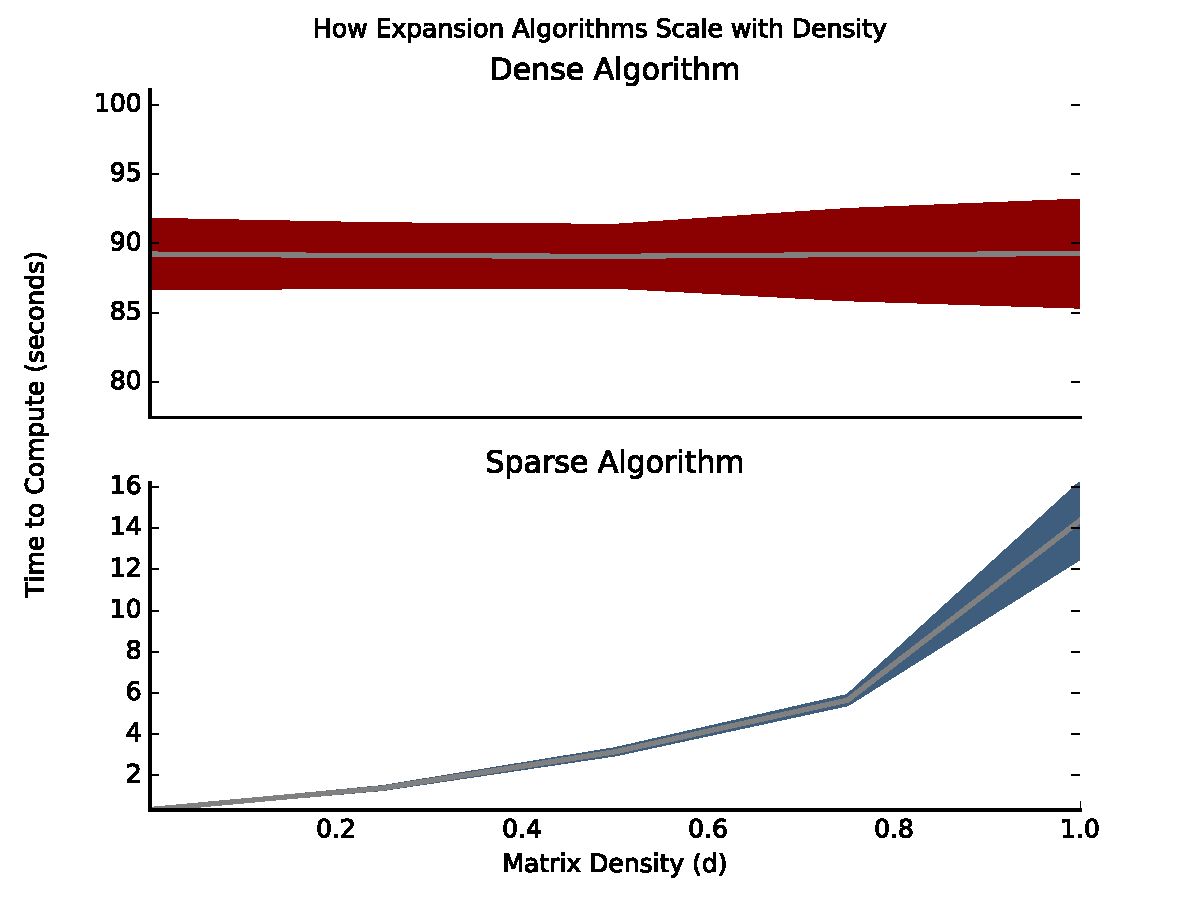
\includegraphics[scale=0.6]{density_vs_time}
    \caption{This plot shows how our algorithm (bottom) scales with the density of a matrix compared to a traditional polynomial feature expansion method (top).
             The task was a second degree expansion, which is why the time of our algorithm scales quadratically with the density.}
    \label{fig:benchmark}
\end{figure}

\section{Conclusion}
We have developed an algorithm for performing polynomial feature expansions on CSR matrices that scales polynomially with respect to the density of the matrix.
While the areas within machine learning this work touches are not en vogue, they are workhorses of industry.
This improvement could therefore spare the burning of much fossil fuel.

\bibliography{sparse_poly}
\bibliographystyle{iclr2017_conference}

\end{document}
